\section{The Front-End Unit} 
\label{feu}
Here we give a brief description of the structure of the Front-End Unit and provide informations needed to make sure it runs in a proper state and identify possible problems if should be encountered. 

\subsection{Unit Set-Up}
The unit should be fixed to the corresponding antenna pole as shown in Fig. \ref{fig:casing}: the front pannel is vertical, with the pressure valve facing ground. 

\begin{figure}[t!]
\begin{center}
{
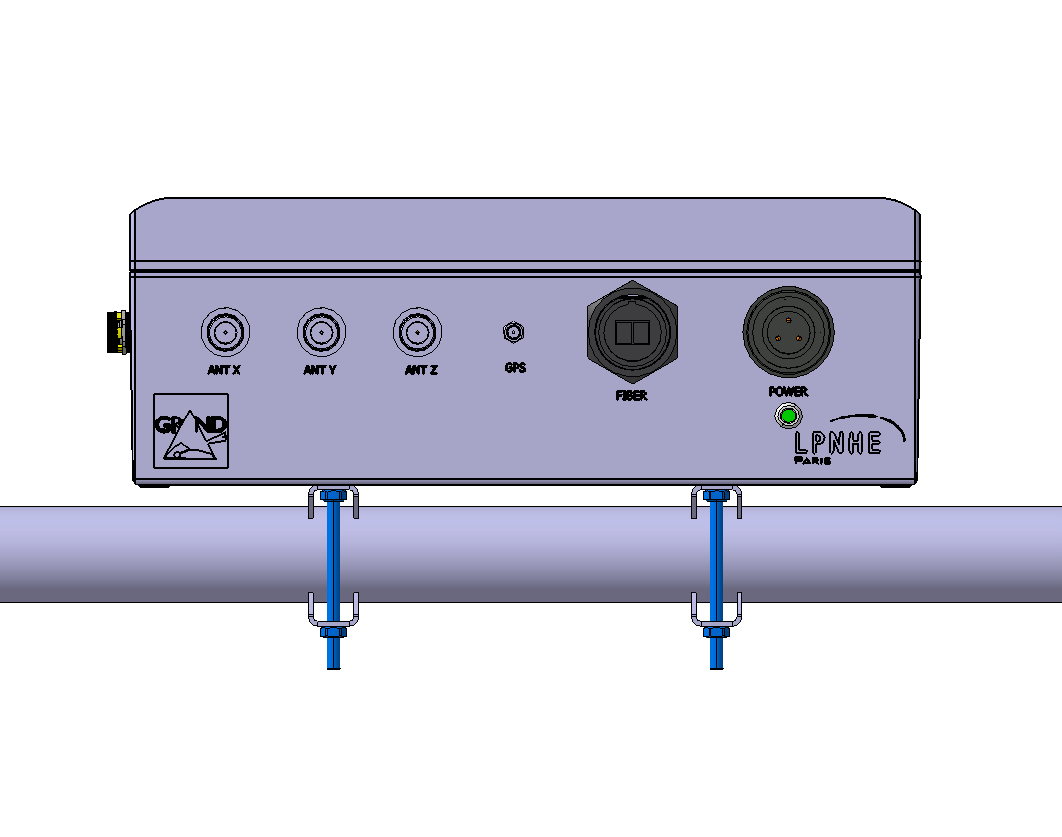
\includegraphics[width=6.5cm,angle=90]{plots/casing.jpg}  
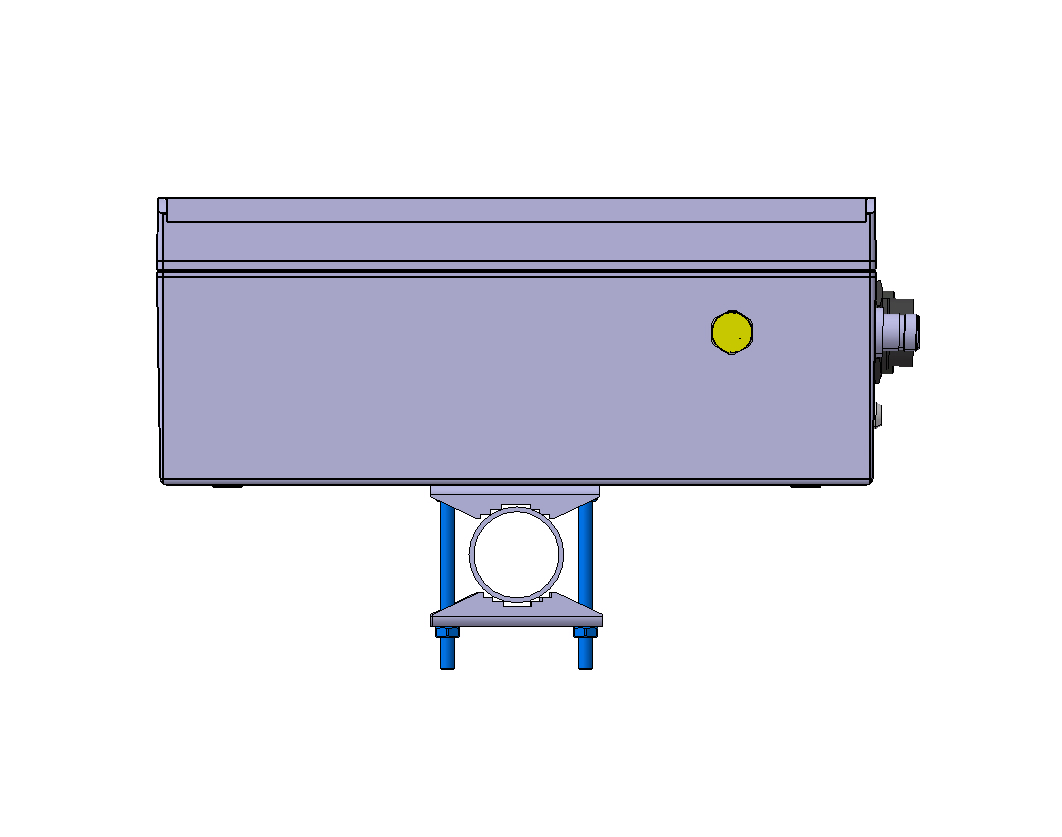
\includegraphics[width=6.5cm,angle=90]{plots/casing_bottom.jpg} 
}
\end{center}
\caption{Front (left) and bottom (right) views of a GRANDproto35 Front-End unit casing once fixed to an antenna pole. 
}
\label{fig:casing} 
G\end{figure}


\subsection{Connections}
\label{connection}
Connections to the Front-End Units should be carried out in the following order:
\begin{enumerate}[i)]
\item {First connect the three outputs of the antenna to the associated inputs {\it ANT X}, {\it ANT Y}, {\it ANT Z} of the Front End Units with the three dedicated coax cables. \hl{Make sure here that you connect the 75$\Omega$ F-type connector end (the thinner one), and not the 50$\Omega$ one (thicker). Inversion would destroy the plug.} Also since the 12\,V DC power supply to the antenna LNAs is provided through these cables, it is in principle safer to plug/unplugg them only when the Front-End Unit power is off. }
\item {Then connect the GPS antenna. \hl{By no means should the GPS antenna be connected when the power is on}. This may destroy the GPS unit inside the board (see section \ref{digital}) and make it unusable. The GPS antenna should preferably be placed above ground. A magnet inside the GPS antenna allows to fix it to a {\bf close-by metalic surface}. }
\item {Then connect the optical fiber (which can however be plugged/unplugged at any time, with no risk of damage). }
\item {Finally plug the power cable. Nominal value of the power supply should be 15\,V, but values between {\bf xx and xx} are still OK. A green LED on the front panel just below the power plug allows to check if the board is powered on.}
\end{enumerate}

\subsection{Front-end board description}
A picture of the board is shown in figure \ref{fig:board}. It can be divided in 4 functionnal sections: analog, digitial, communication and power supply.

\begin{figure}[t!]
\begin{center}
{
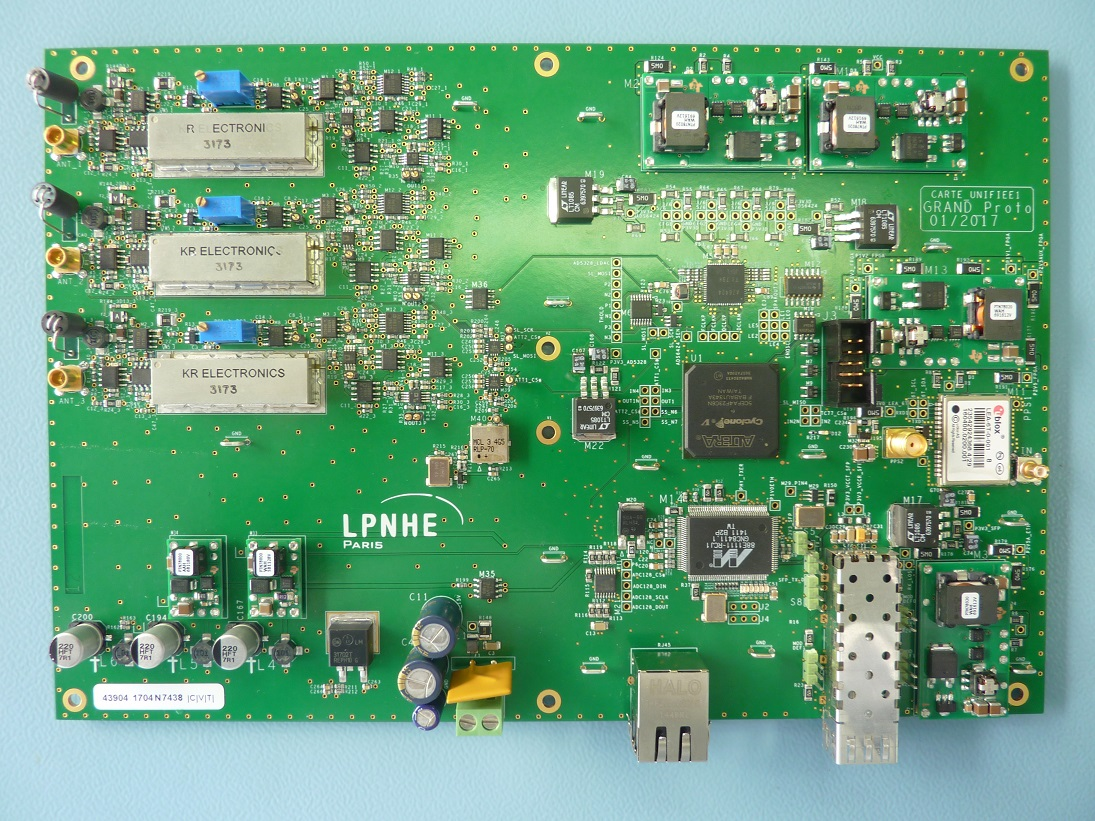
\includegraphics[width=\textwidth]{plots/board.jpg}  
}
\end{center}
\caption{Picture of the GRANDproto35 Front-End unit board. TO BE UPDATED.
}
\label{fig:board} 
\end{figure}


\subsubsection{Analog part}
\label{analog}
The description of the analog part of the board is given in details in \cite{GP35ana} (in French). Here we just give a brief overview. \\
%
The analog part lies in the top-left corner of the board. Signal input to the board is done for each of the three channels through an MMCX 75$\Omega$ jack connected to the corresponding F-type connector. From top to bottom we have X, Y and Z channels. The signal is adapted to a 50$\Omega$ impedance thanks to a dedicated amplifier placed just after the connector, then fed into the 30-100\,MHz filters tagged {\it KR ELECTRONICS}. Signal is finally processed through a power detector AD8310 \cite{AD8310}, which acts as an envelop detector. The power detector runs in differential mode. Its common mode voltage has a nominal value of 0.9\,V adjusted thanks to a potentiometer (blue square, just above the filter). It can be measured between ground and the test point shown on Fig. \ref{fig:board} {\bf To Be Done}. \\
%
The analog section also provides the power supply to the LNAs placed inside the antenna nut through a bias-tee system connected to the MMCX plugs. \hl{This means that in normal operation, a 12\,V DC voltage is applied to the input plugs, which the user should be aware of when performing tests on a powered board.} The LNAs power supply can be switched on and off by the user (see section \ref{TRENDDAQ}).  \\
%
In addition to this, the analog part includes a trigger section, where the signals at the output of the filters are compared to threshold values. A trigger flag is generated and sent to the FPGA (see section \ref{digital}) if one channel exceeds it. Note that there are six independant trigger channels, with two polarities for each of the three channels. The user can activate/inhibit independantly each of these trigger channels and set their respective threshold values (see section \ref{TRENDTRIG}). \\
%
Finaly an internal calibration system is also included in this analog part: its core is a 66.666\,MHz quartz oscillator (placed at the center of the board), which generates a sine wave. Its amplitude can be moderated thanks to two attenuators, with attenuation values adjustable by the user (see section \ref{TRENDDAQ}). When the user uses the DAQ in calibration mode, the input of the signal treatment chain detailed above is switched from the MMCX connector input to this calibration signal.
   

\subsubsection{Digital part}
\label{digital}
The digital treatment of the signal is detailed in \cite{GP35daq}. It is performed on the right part of the card, starting with a 4-channels ADC \cite{ADCdoc} running at a nominal frequency of 50\,MHz, ajustable up to 100\,MHz through the FPGA firmware. The ADC continously digitizes the signal coming from the three analog channels. The 4$^{th}$ ADC channel is used in calibration mode to digitize the signal at the output of the quartz oscillator. The digital signal of each of the four channels is buffered in a circular register inside the FPGA. When one trigger is received (see previous section), a subset of length 2$\times${\it OFFSET} (where {\it OFFSET} is a parameter set by the user at run start) is saved for each of the four channels to form one event. A GPS time-tag is also requested to the uBlox GPS unit\cite{GPS} and embeded in the event header and sent to the board output (see section \ref{comms}).

\subsubsection{Communication}
\label{comms}
Communication with the DAQ computer is done through a Marvell interface chip, using the GEDEK Communication Engine. Messages are exchanged using UDP protocol. Either a standard ethernet plug can be used, or optical transfer through an SFP connector (see FIg. \ref{fig:board}). A jumper placed just below the Marvell chip allows to switch from one to the other (left: ethernet plug, right: optical). The latter is the standard communication system in GRANDproto35 operation, with a bi-modal SFP ($\lambda_1$ = 1310\,nm \& $\lambda_2$ = 1550\,nm) allowing down (data) and upstream (commands) communication on a single fiber. \\
%
The Front-End Unit is identified through a unique MAC adress given by a specific chip (Dallas DS2502). At boot time, IP adresses of all units are identically set to 192.168.1.18 by default.  A software program however allows to map each MAC adress to an IP adress of format 192.168.1.1xx (see section \ref{startup}) where xx is the Front-End unit ID, ranging between 01 and 35. This IP adress is used for any further communication with the DAQ PC, whose IP should be 192.168.1.1 within a local network.


\subsubsection{Power supply}
The nominal power supply of the Front-End Unit is 15\,V DC, and standard power consumption is $\sim$10W in normal run conditions. In standard operation at Ulastai, this DC voltage is provided by the external AC/DC converter installed at the pod level. There is also an internal AC/DC converter fixed on the internal side of the Front-End unit casing, but it is not used. \\
%
A re-armable fuse is installed at the input of the board power supply (yellow thing on Fig. \ref{fig:board}). It will disrupt power supply in case a current surge is detected ({\bf level ?}). It is re-armed after power cycling. \\
%
DC voltages of +4\,V and -3.3\,V are generated by DC-DC converters located on small mezanines placed at 3 corners of the board.

\subsubsection{Board control}
\label{control}
There are several tools to check that the board is in a proper state and identify possible issues. \\
%

 {\bf TO BE COMPLETED WITH INPUT FROM LPNHE COLLEAGUES.}
